\subsection{System Evaluation}~\label{exp:sys_eval}
We evaluate the proposed framework from three perspectives. We first examine how the confidence threshold $\tau$ influences the trade-off between task performance and user feedback. We then compare the proposed query strategy with representative baselines under identical task settings. Finally, we analyze the computational scalability of the method as the symbolic state space increases.

\subsubsection{Threshold Ablation}~\label{exp:sys_threshold}
We first evaluate the effect of the confidence threshold $\tau$ on system performance. Fig.~\ref{fig:sys_tau} and Table~\ref{tab:sys_tau} report the resulting success rate, execution steps, and number of user queries across different threshold values.


\begin{figure*}[t!]
    \centering
    \begin{subfigure}[t]{0.48\textwidth}
        \centering
        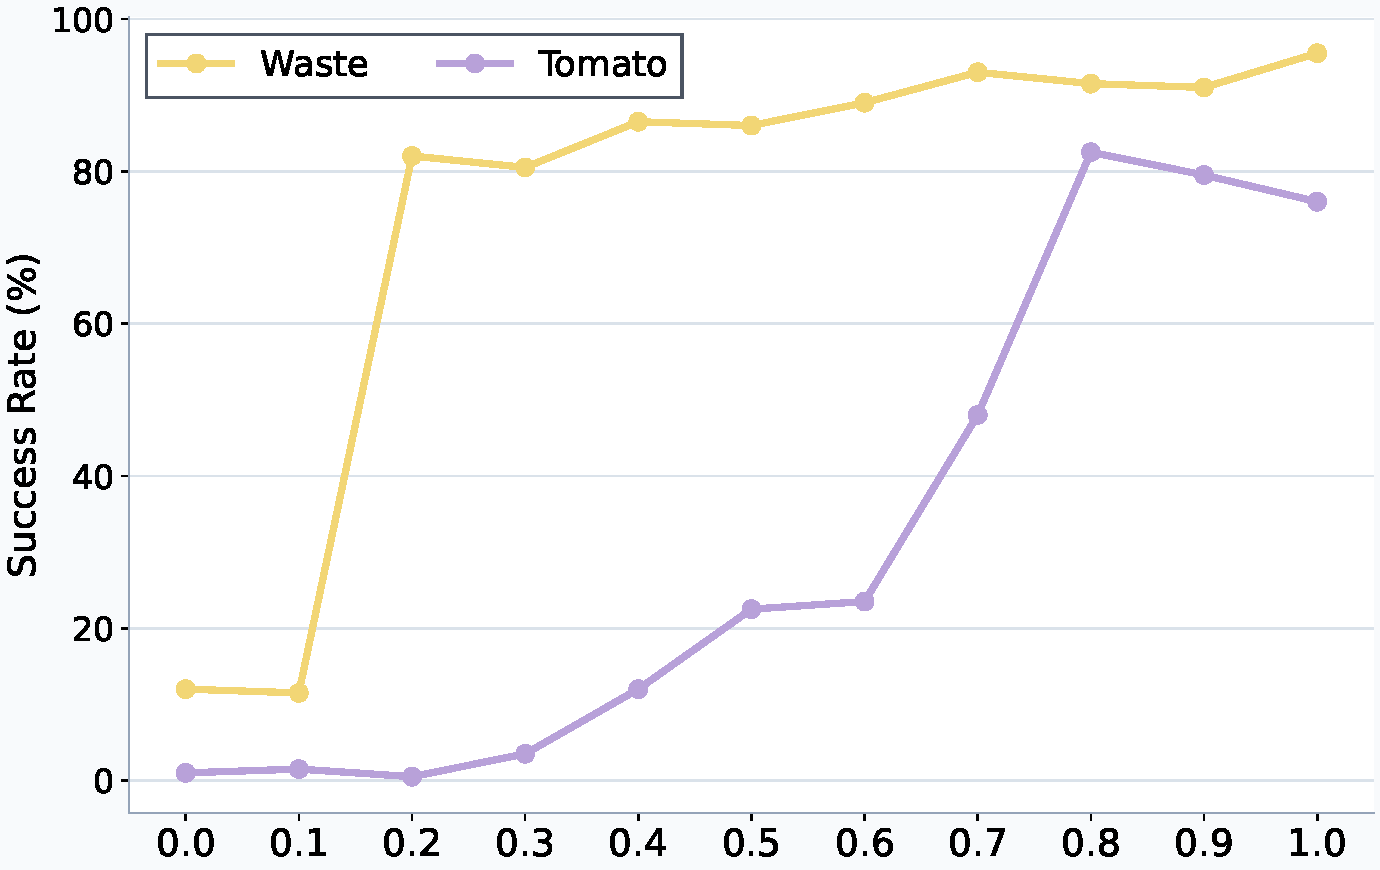
\includegraphics[width=\linewidth]{figures/system_eval/fig_thres_success_rate.pdf}
        \caption{Success rate}
        \label{fig:sys_tau_success}
    \end{subfigure}
    \hfill
    \begin{subfigure}[t]{0.48\textwidth}
        \centering
        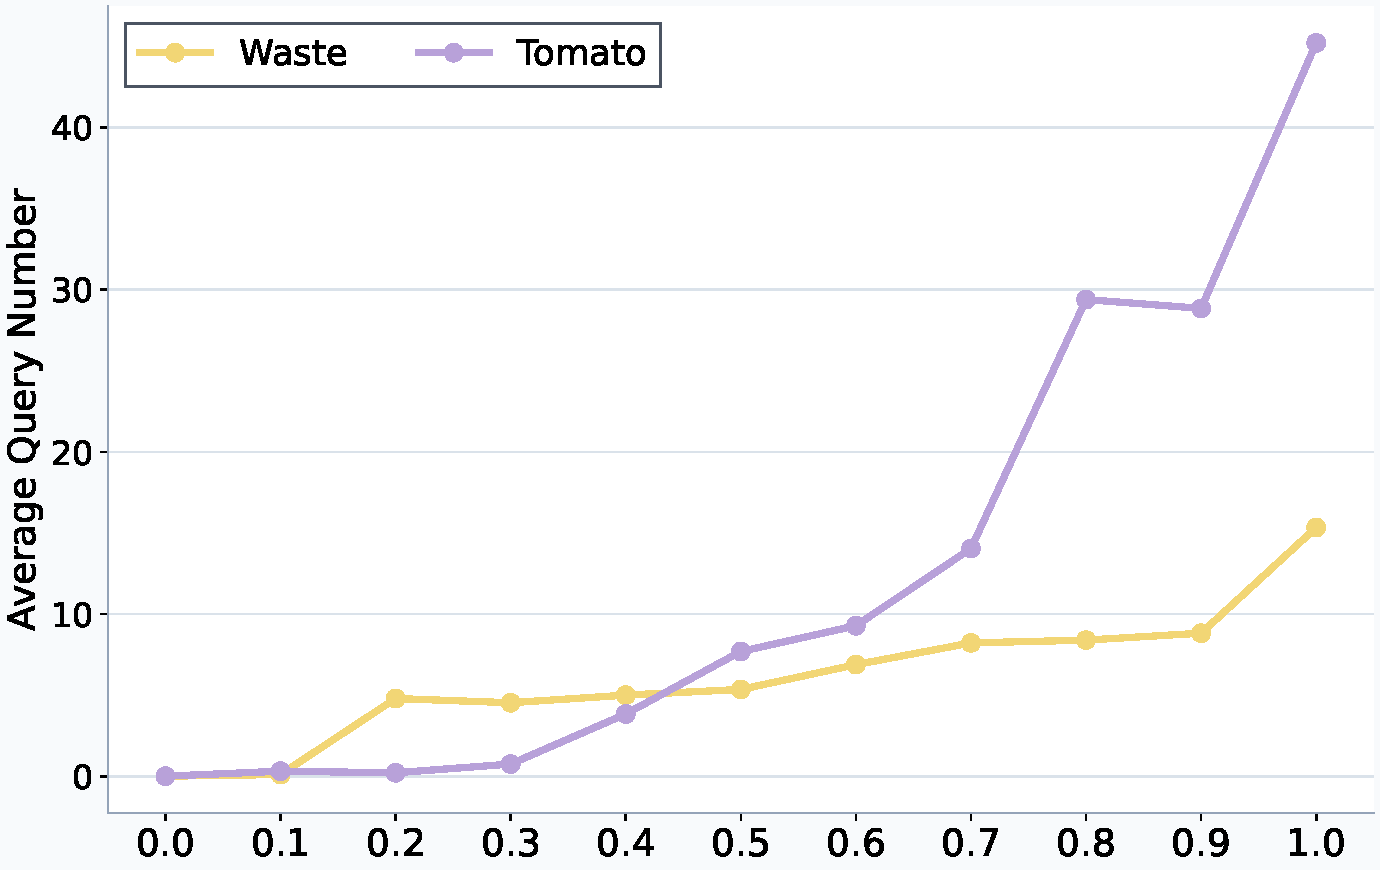
\includegraphics[width=\linewidth]{figures/system_eval/fig_thres_average_question.pdf}
        \caption{Average queries}
        \label{fig:sys_tau_queries}
    \end{subfigure}
    \vspace{0.4em}

    \begin{subfigure}[t]{0.48\textwidth}
        \centering
        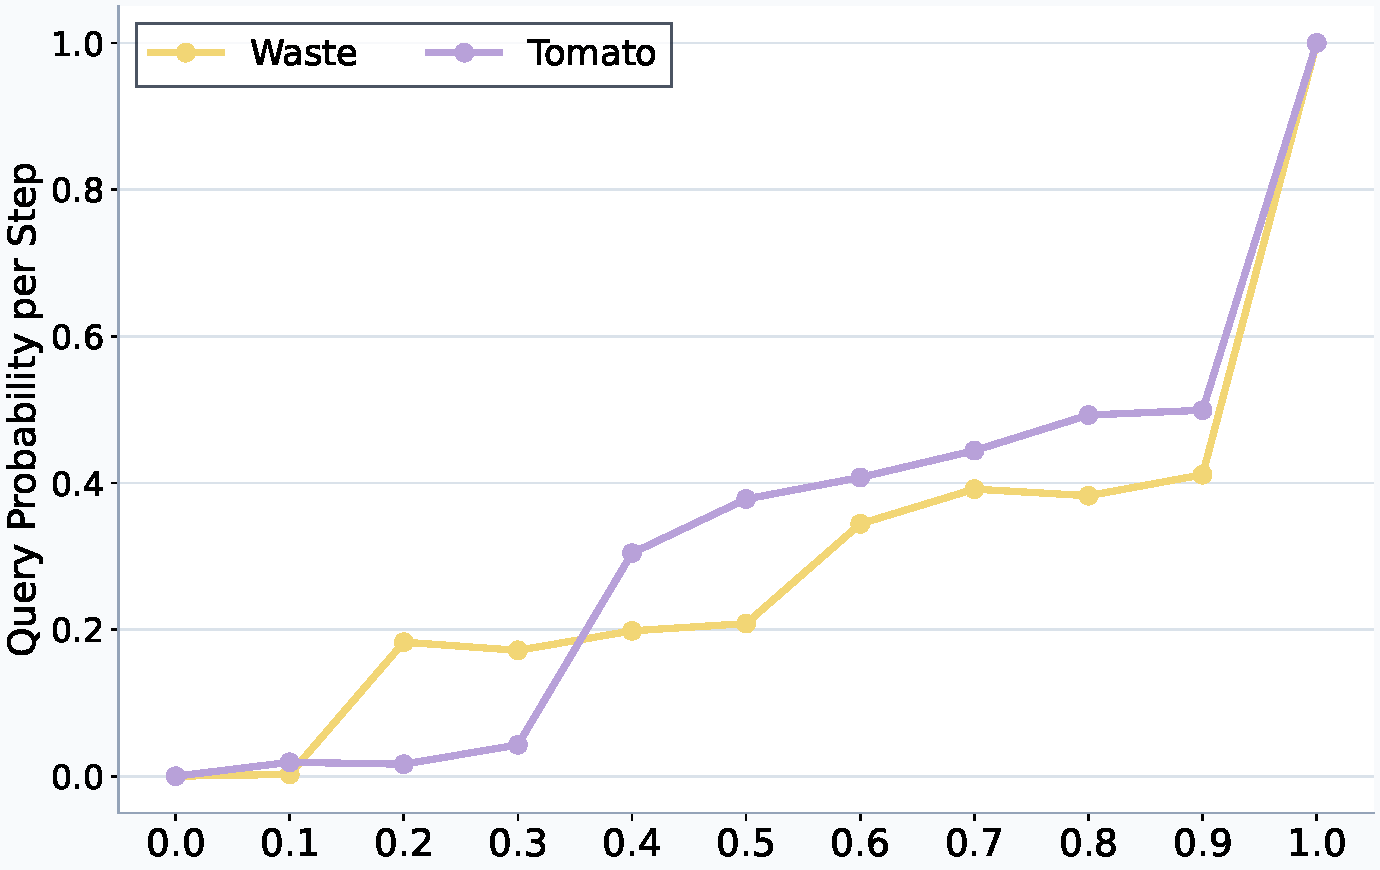
\includegraphics[width=\linewidth]{figures/system_eval/fig_thres_query_probability_per_step.pdf}
        \caption{Query probability}
        \label{fig:sys_tau_query_prob}
    \end{subfigure}
    \hfill
    \begin{subfigure}[t]{0.48\textwidth}
        \centering
        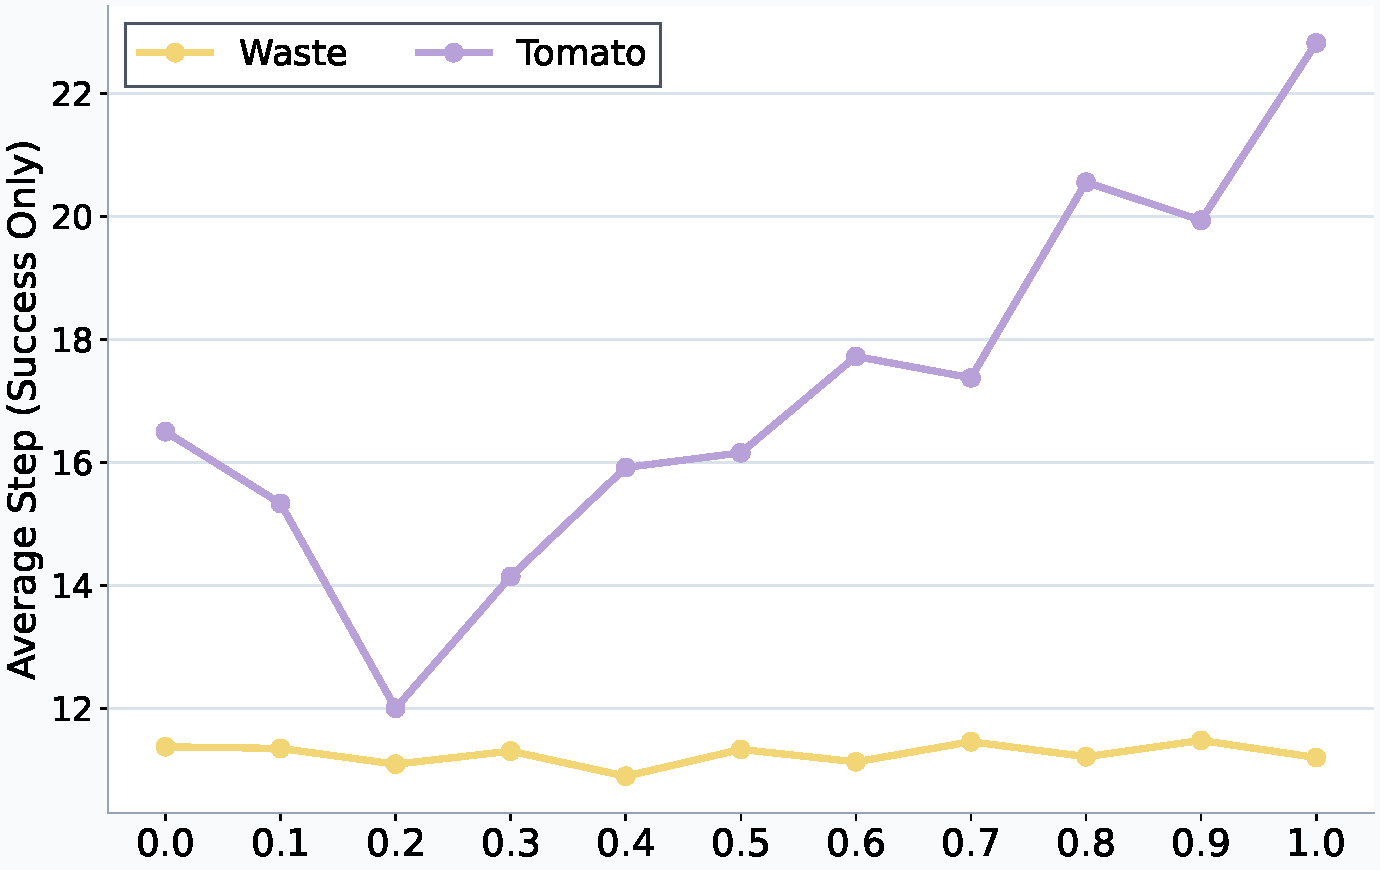
\includegraphics[width=\linewidth]{figures/system_eval/fig_thres_average_step_success_only.pdf}
        \caption{Planning length}
        \label{fig:sys_tau_steps}
    \end{subfigure}
    \caption{Effect of the confidence threshold $\tau$ on system behavior. (a) Task success rate. (b) Average number of questions per episode. (c) Query probability per execution step. (d) Planning length for successful runs. Increasing $\tau$ generally increases feedback, but very high thresholds can add interaction without improving success.}
    \label{fig:sys_tau}
\end{figure*}

\begin{table*}[t]
\centering
\caption{Threshold sensitivity for all evaluated values of $\tau$. Success rates are percentages. Query counts are average questions per episode, query rate is the fraction of execution steps with at least one question, and average steps are computed over successful runs. Each domain-threshold cell aggregates $200$ episodes.}
\label{tab:sys_tau}
\footnotesize
\setlength{\tabcolsep}{2pt}
\begin{tabular*}{\textwidth}{@{\extracolsep{\fill}}lcccccccc}
\toprule
\multirow{2}{*}{$\boldsymbol{\tau}$} & \multicolumn{4}{c}{\textbf{Waste Sorting}} & \multicolumn{4}{c}{\textbf{Tomato Harvesting}} \\
\cmidrule(lr){2-5}\cmidrule(lr){6-9}
& \textbf{Success Rate (\%)} & \textbf{Avg. Queries} & \textbf{Query Rate} & \textbf{Avg. Steps} & \textbf{Success Rate (\%)} & \textbf{Avg. Queries} & \textbf{Query Rate} & \textbf{Avg. Steps} \\
\midrule
0.0 & 12.0 & 0.0 & 0.00 & 11.4 & 1.0 & 0.0 & 0.00 & 16.5 \\
0.1 & 11.5 & 0.1 & 0.00 & 11.3 & 1.5 & 0.3 & 0.02 & 15.3 \\
0.2 & 82.0 & 4.8 & 0.18 & 11.1 & 0.5 & 0.2 & 0.02 & 12.0 \\
0.3 & 80.5 & 4.5 & 0.17 & 11.3 & 3.5 & 0.8 & 0.04 & 14.1 \\
0.4 & 86.5 & 5.0 & 0.20 & 10.9 & 12.0 & 3.8 & 0.30 & 15.9 \\
0.5 & 86.0 & 5.4 & 0.21 & 11.3 & 22.5 & 7.7 & 0.38 & 16.2 \\
0.6 & 89.0 & 6.9 & 0.34 & 11.1 & 23.5 & 9.3 & 0.41 & 17.7 \\
0.7 & 93.0 & 8.2 & 0.39 & 11.5 & 48.0 & 14.0 & 0.44 & 17.4 \\
0.8 & 91.5 & 8.4 & 0.38 & 11.2 & 82.5 & 29.4 & 0.49 & 20.6 \\
0.9 & 91.0 & 8.8 & 0.41 & 11.5 & 79.5 & 28.8 & 0.50 & 19.9 \\
1.0 & 95.5 & 15.3 & 1.00 & 11.2 & 76.0 & 45.2 & 1.00 & 22.8 \\
\bottomrule
\end{tabular*}
\end{table*}

The results show that the two domains respond differently to the confidence threshold. In waste sorting, performance improves rapidly once a small amount of uncertainty is resolved, increasing from $11.5\%$ at $\tau=0.1$ to $82.0\%$ at $\tau=0.2$. Because task success primarily depends on identifying the correct waste category, additional feedback provides limited benefit once the category is determined. In contrast, tomato harvesting involves a longer sequence of dependent decisions, including navigation, detection, picking, scanning, and execution. Unresolved uncertainty can therefore propagate through multiple stages of the task, causing performance to remain low at small threshold values. Success increases substantially only at higher thresholds and reaches $82.5\%$ at $\tau=0.8$.

Increasing $\tau$ consistently increases interaction because the planner requests feedback for a larger fraction of uncertain beliefs. This trend is reflected in both the average number of queries and the query rate. However, the additional interaction does not always translate into higher task success. In tomato harvesting, increasing the threshold from $\tau=0.8$ to $\tau=1.0$ increases the average number of queries from $29.4$ to $45.2$ and the query rate from $0.49$ to $1.00$, while success decreases from $82.5\%$ to $76.0\%$. This suggests that over-querying can introduce unnecessary interaction and may expose the belief update to additional noisy corrections without improving downstream decisions. In waste sorting, by contrast, the simpler category-assignment structure benefits from high confidence and reaches $95.5\%$ at $\tau=1.0$. Based on the cross-domain trade-off between success and interaction cost, we use $\tau=0.8$ in the remaining experiments.



\subsubsection{Baseline Comparison}~\label{exp:sys_baseline}
We next compare the proposed query strategy with representative alternatives. \textbf{All} requests feedback whenever multiple frontier hypotheses remain, regardless of the current confidence level. \textbf{No} performs autonomous execution without user feedback. \textbf{Random} requests state-level feedback at randomly selected decision points. \textbf{KnowNo}~\cite{ren2023robots} represents an action-level query baseline that asks the user to choose among candidate next actions.


We use an oracle user in the system evaluation. For state-level query policies, the oracle returns the correct truth value for each queried hypothesis. To isolate query timing, \textbf{Random} uses the same query rates as \textbf{Ours} at $\tau=0.8$, with rates of $0.38$ in waste sorting and $0.48$ in tomato harvesting. When a query is triggered, it uses the same state-level query construction, belief filtering, and planning procedure as \textbf{Ours}. For \textbf{KnowNo}, the oracle selects the correct action if it appears in the generated candidate set. If no generated candidate is correct, the oracle selects an option indicating that the correct action is not in the list. We also distinguish \textbf{All} from the $\tau=1.0$ setting. The \textbf{All} policy requests feedback whenever multiple frontier hypotheses remain, whereas $\tau=1.0$ continues querying until complete confidence is achieved. Consequently, \textbf{All} may terminate querying even when uncertainty remains, while $\tau=1.0$ attempts to eliminate all uncertainty before acting.


\begin{figure*}[t!]
    \centering
    \begin{subfigure}[t]{0.48\textwidth}
        \centering
        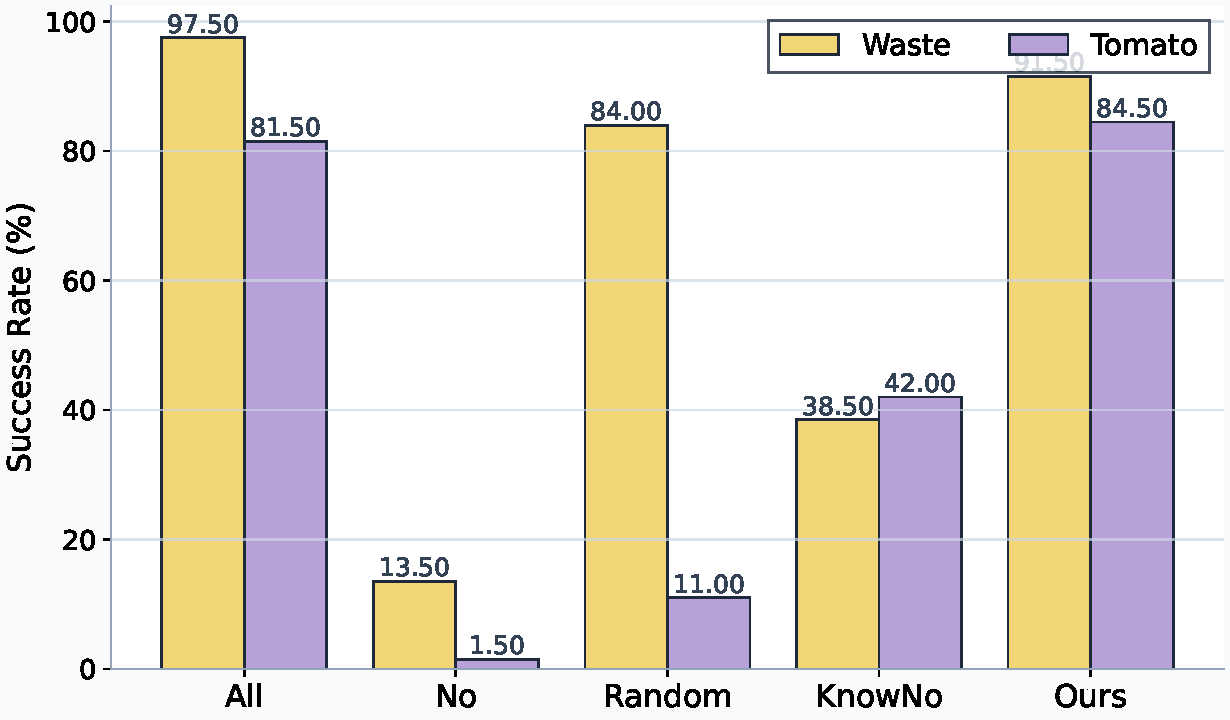
\includegraphics[width=\linewidth]{figures/system_eval/fig_ablation_success_rate.pdf}
        \caption{Success rate}
        \label{fig:sys_baseline_success}
    \end{subfigure}
    \hfill
    \begin{subfigure}[t]{0.48\textwidth}
        \centering
        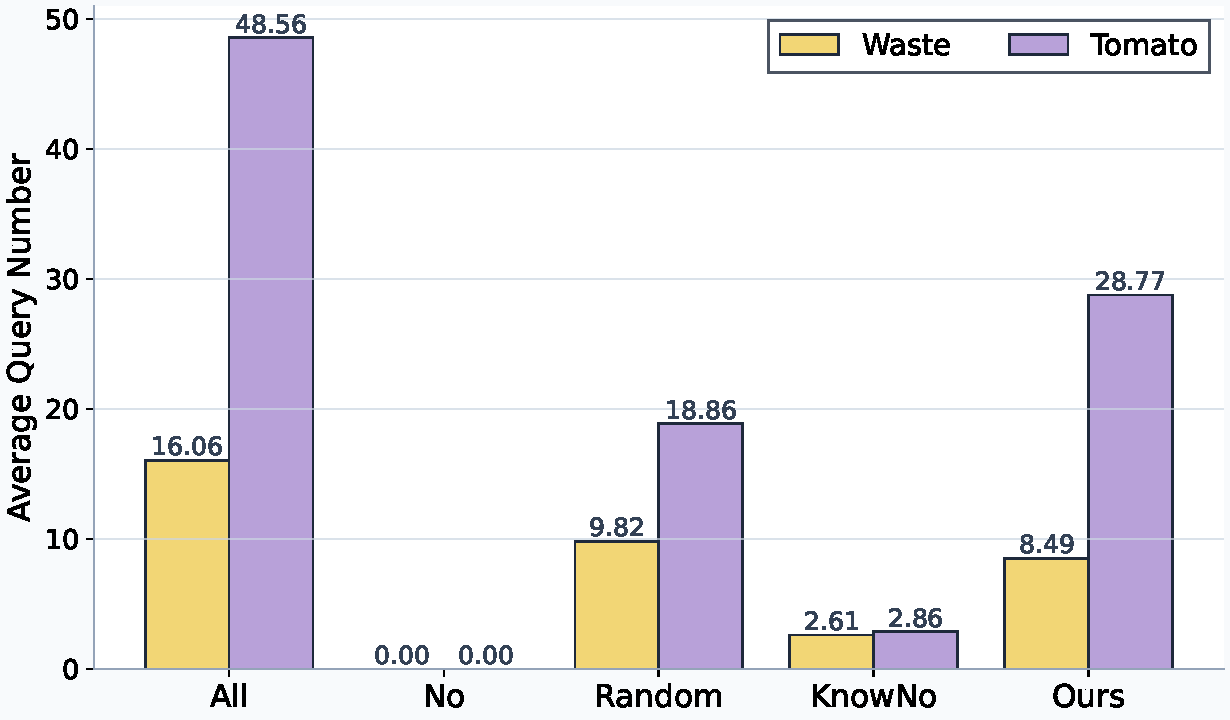
\includegraphics[width=\linewidth]{figures/system_eval/fig_ablation_average_question_success_only.pdf}
        \caption{Average queries}
        \label{fig:sys_baseline_queries}
    \end{subfigure}
    \vspace{0.4em}

    \begin{subfigure}[t]{0.48\textwidth}
        \centering
        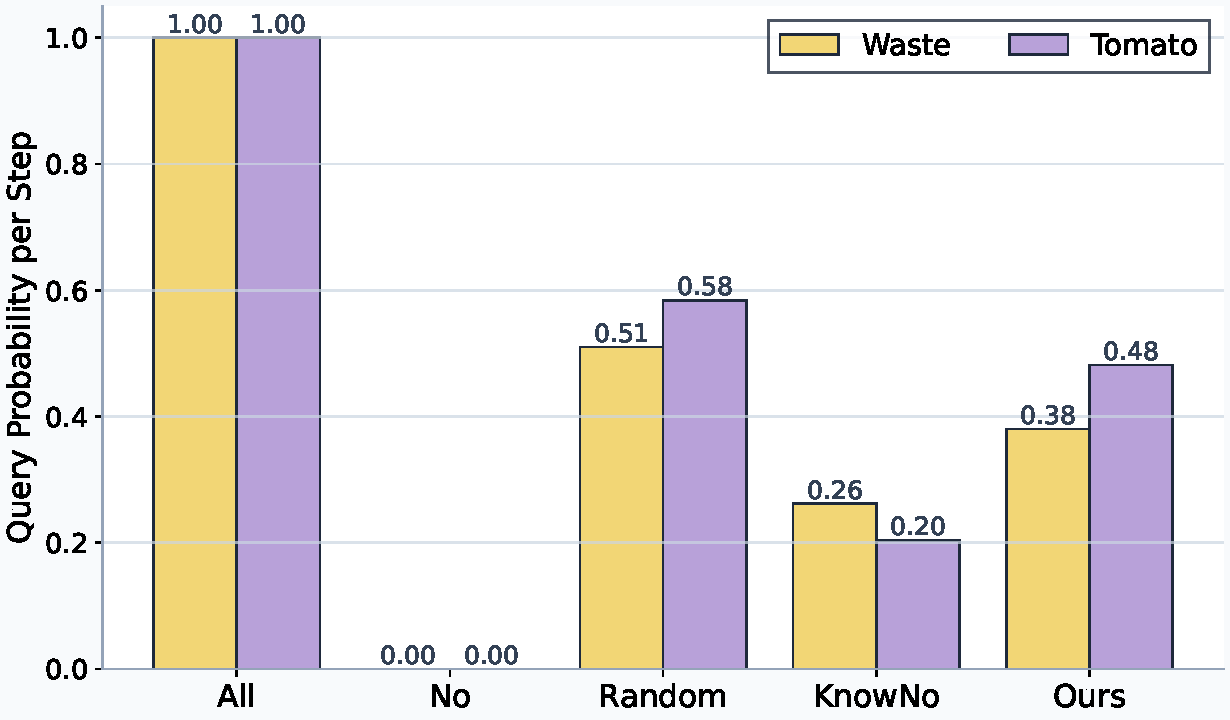
\includegraphics[width=\linewidth]{figures/system_eval/fig_ablation_query_probability_per_step_success_only.pdf}
        \caption{Query rate}
        \label{fig:sys_baseline_query_rate}
    \end{subfigure}
    \hfill
    \begin{subfigure}[t]{0.48\textwidth}
        \centering
        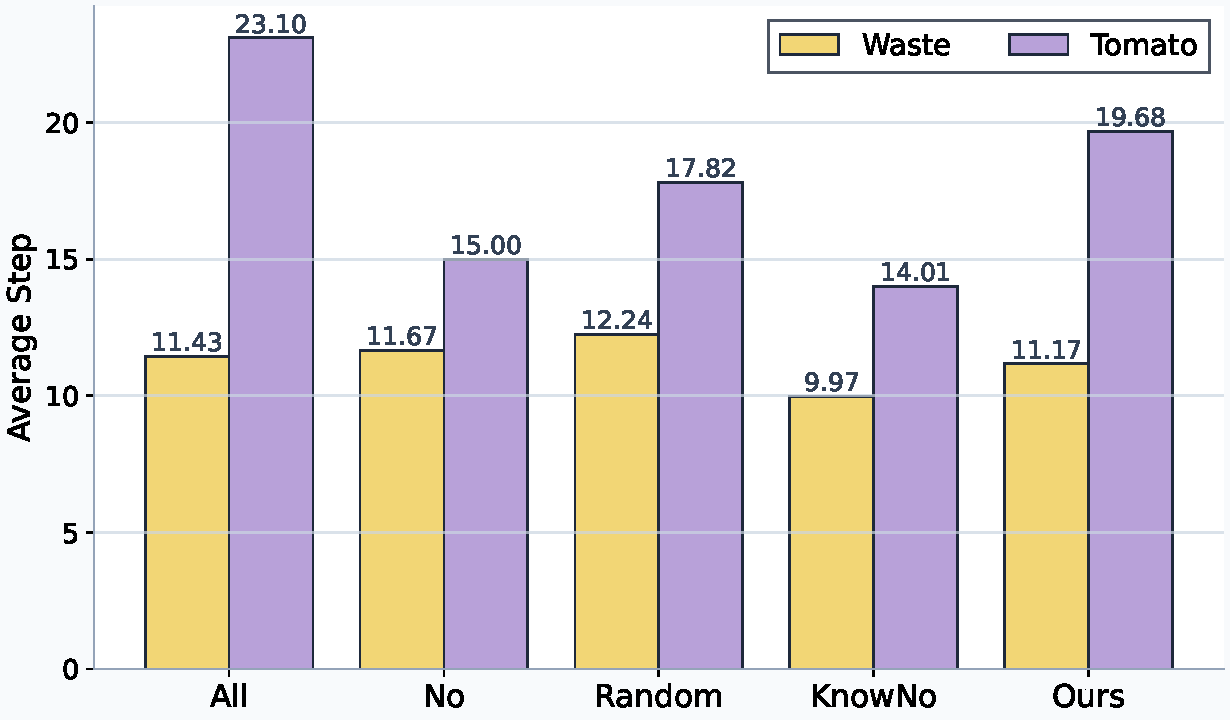
\includegraphics[width=\linewidth]{figures/system_eval/fig_ablation_average_step_success_only.pdf}
        \caption{Planning length}
        \label{fig:sys_baseline_steps}
    \end{subfigure}
    \caption{Baseline comparison at $\tau=0.8$. (a) Task success rate. (b) Average number of questions in successful runs. (c) Query rate, computed as the fraction of successful-run execution steps in which at least one question is asked. (d) Planning length for successful runs. The proposed policy preserves high task success while asking substantially fewer questions than dense supervision.}
    \label{fig:sys_baseline}
\end{figure*}

\begin{table*}[t]
\centering
\caption{Baseline comparison at $\tau=0.8$. Average queries, query rate, and average steps are computed over successful runs to compare the interaction cost of completed tasks.}
\label{tab:system_eval}
\footnotesize
\setlength{\tabcolsep}{2pt}
\begin{tabular*}{\textwidth}{@{\extracolsep{\fill}}lcccccccc}
\toprule
\multirow{2}{*}{\textbf{Condition}} & \multicolumn{4}{c}{\textbf{Waste Sorting}} & \multicolumn{4}{c}{\textbf{Tomato Harvesting}} \\
\cmidrule(lr){2-5}\cmidrule(lr){6-9}
& \textbf{Success Rate (\%)} & \textbf{Avg. Queries} & \textbf{Query Rate} & \textbf{Avg. Steps} & \textbf{Success Rate (\%)} & \textbf{Avg. Queries} & \textbf{Query Rate} & \textbf{Avg. Steps} \\
\midrule
\textbf{All}    & \textbf{97.5} & 16.1 & 1.00 & 11.4 & 81.5 & 48.6 & 1.00 & 23.1 \\
\textbf{No}     & 13.5 & 0.0  & 0.00 & 11.7 & 1.5  & 0.0  & 0.00 & 15.0 \\
\textbf{Random} & 84.0 & 9.8  & 0.51 & 12.2 & 11.0 & 18.9 & 0.58 & 17.8 \\
\textbf{KnowNo} & 38.5 & \textbf{2.6}  & \textbf{0.26} & \textbf{10.0} & 42.0 & \textbf{2.9}  & \textbf{0.20} & \textbf{14.0} \\
\textbf{Ours}   & 91.5 & 8.5  & 0.38 & 11.2 & \textbf{84.5} & 28.8 & 0.48 & 19.7 \\
\bottomrule
\end{tabular*}
\end{table*}


\textbf{All} achieves high success rates in both domains, reaching $97.5\%$ in waste sorting and $81.5\%$ in tomato harvesting. This comes with frequent interaction, with average query counts of $16.1$ and $48.6$ and a query rate of $1.00$ in both domains. \textbf{No} performs poorly, achieving $13.5\%$ success in waste sorting and $1.5\%$ in tomato harvesting. \textbf{Random} reaches $84.0\%$ success in waste sorting, but remains low in tomato harvesting at $11.0\%$.

The difference between the two \textbf{Random} results follows the structure of the domains. In waste sorting, most uncertain facts concern object categories, and a category fact directly determines the corresponding bin. Once the category is resolved, the remaining pick and place sequence is mostly determined by whether the object is grasped. In tomato harvesting, the detect and scan stages are tied to decisions that can lead to dead ends. Ripe and rotten tomatoes may remain ambiguous after detection, and the robot must scan a picked tomato before deciding whether to place or discard it. If this ambiguity is not resolved at the relevant stage, the planner may commit to a place or discard action before the tomato state is properly disambiguated.

In contrast, \textbf{Ours} provides a favorable balance between task success and interaction cost. In waste sorting, it reduces the average number of queries from $16.1$ to $8.5$, with a success-rate decrease from $97.5\%$ for \textbf{All} to $91.5\%$ for \textbf{Ours}. In tomato harvesting, \textbf{Ours} achieves $84.5\%$ success compared with $81.5\%$ for \textbf{All}, while reducing the average number of queries from $48.6$ to $28.8$. This indicates that the selected queries capture uncertainty at decision points such as detect and scan, where unresolved state ambiguity can change the subsequent place or discard decision. The query rates of $0.38$ and $0.48$ also show that these points can be handled without querying at every execution step.


\textbf{KnowNo} uses substantially fewer queries than \textbf{Ours}, requiring $2.6$ queries instead of $8.5$ in waste sorting and $2.9$ instead of $28.8$ in tomato harvesting. It also records shorter successful execution sequences, with average planning lengths of $10.0$ and $14.0$ steps compared with $11.2$ and $19.7$ for \textbf{Ours}. These numbers reflect the role of action-level feedback. Once the correct action is available among the candidates, selecting it can directly advance the execution without additional state verification.


The success rates of \textbf{KnowNo}, however, remain limited to $38.5\%$ and $42.0\%$, while \textbf{Ours} achieves $91.5\%$ and $84.5\%$ in the same domains. Since the action candidates are conditioned on the perceived state, an overconfident but incorrect state estimate can produce an action set that does not contain the action that is correct under the true state. \textbf{Ours} fails for a different reason. The oracle provides correct truth values for state queries, so remaining failures mainly arise from the planner after the belief has been filtered. Typical cases include repeated actions that do not make progress, or dead-end sequences in tomato harvesting where the planner commits to place or discard before the scan-related ambiguity has been resolved. Thus, the two methods fail at different points in the pipeline. \textbf{KnowNo} can fail before action selection because the correct action is absent from the candidate set, whereas \textbf{Ours} can fail after correct state feedback due to limitations of the POMCP-based planner. We report the KnowNo implementation details in Appendix~\ref{appx:exp}.


\subsubsection{Scalability Test}~\label{exp:sys_scale}
We next examine whether the proposed framework remains effective as task complexity increases. The original setting contains four objects per domain. The scaled setting contains six objects in both domains, increasing the symbolic belief space, the number of possible object assignments, and the planning complexity. We keep the policy fixed to \textbf{Ours} with $\tau=0.8$ and increase the maximum planning horizon to accommodate the longer task sequences.


\begin{table}[t]
\centering
\caption{Scalability results for \textbf{Ours} on six-object scenes. Values are means over $200$ scaled episodes per domain.}
\label{tab:sys_scale}
\footnotesize
\setlength{\tabcolsep}{0pt}
\begin{tabular*}{\columnwidth}{@{\extracolsep{\fill}}lcccc}
\toprule
\multirow{2}{*}{\textbf{Metric}} & \multicolumn{2}{c}{\textbf{Waste}} & \multicolumn{2}{c}{\textbf{Tomato}} \\
\cmidrule(lr){2-3}\cmidrule(lr){4-5}
& \textbf{Orig.} & \textbf{Scale} & \textbf{Orig.} & \textbf{Scale} \\
\midrule
Success (\%)        & 91.5 & 92.0 & 84.5 & 74.0 \\
Avg. steps          & 11.2 & 15.3 & 19.7 & 33.1 \\
Avg. queries        & 8.3  & 11.3 & 27.3 & 80.6 \\
Query rate          & 0.38 & 0.33 & 0.48 & 0.54 \\
Episode time (s)    & 5.3  & 22.9 & 56.0 & 159.9 \\
\bottomrule
\end{tabular*}
\end{table}

The scaled waste sorting results show that the proposed framework remains effective as the number of objects increases from four to six. The success rate remains nearly unchanged at approximately $92.0\%$, while the average plan length increases from $11.2$ to $15.3$ steps. The average number of queries also increases from $8.3$ to $11.3$. However, the query rate decreases slightly from $0.38$ to $0.33$, indicating that the additional objects primarily increase task length rather than the fraction of decision points that require feedback.

The tomato harvesting domain presents a more challenging scalability test because uncertainty is distributed across multiple state variables, including object identity, stem location, ripeness, scan outcomes, and grasped objects. As the number of tomatoes increases, the success rate decreases from $84.5\%$ to $74.0\%$, while the average plan length increases from $19.7$ to $33.1$ steps. The average number of queries also rises from $27.3$ to $80.6$. Despite this increase, the query rate changes only moderately from $0.48$ to $0.54$. This result suggests that the policy continues to request feedback selectively rather than querying at every decision step. The primary scalability cost appears in planning and belief maintenance, as reflected by the increase in episode execution time from $56.0$ to $159.9$ seconds.

Overall, the scalability results suggest that the proposed policy extends to larger symbolic scenes while preserving its selective feedback mechanism. As task complexity increases, the method requires more interaction in the harder tomato domain, but the query rate increases only moderately and does not collapse into dense supervision.


\subsubsection{System Discussion}~\label{exp:sys_discuss}
The system evaluation returns to the two questions that motivate our framework. When should the robot ask for feedback, and what should the user be asked to provide? The results suggest that both decisions should depend on which state uncertainty affects planning at each step.

The threshold experiment shows that more feedback is not always better. Low thresholds leave important uncertainty unresolved and lead to poor task performance. High thresholds increase the number of questions but do not provide proportional gains in success rate. The strongest results are obtained when feedback is requested for uncertainty that is likely to affect future planning decisions.

The baseline comparison examines the two parts of the proposed query policy separately. \textbf{All} shows the effect of dense state verification, achieving high success rates with frequent interaction. \textbf{Random} uses the same query rates as \textbf{Ours}, but triggers state verification at randomly selected decision points. Its low success in tomato harvesting shows that feedback must arrive before state ambiguity leads the planner into an irreversible decision. \textbf{KnowNo} changes the form of feedback by asking the user to choose the next action. This keeps the number of queries small if the correct action is included among the choices. In our system-level evaluation, the choices are generated from the perceived state, so an overconfident but incorrect perception can remove the true-state action from the candidate set.

These results are consistent with the intended role of feedback in our framework. The user verifies state facts that affect the feasible action space, and the planner uses the updated belief to choose the next action. Human input therefore changes the state estimate that planning depends on, while action selection remains with the robot. This allows the system to use feedback at decision points where state ambiguity affects execution, without querying at every opportunity.

The scalability experiment shows that larger problems primarily increase planning and belief maintenance costs. In the waste sorting domain, performance remains stable as the number of objects increases. In the tomato harvesting domain, the larger belief space leads to longer planning horizons, more queries, and higher computational cost. However, the query rate increases only moderately, indicating that the policy remains selective rather than asking for feedback at every opportunity. These results suggest that the proposed query policy can preserve selective feedback acquisition even as task complexity and belief-space size increase.
